\begin{figure} [!ht]
\begin{center}
\begin{tikzpicture}
	[
	sibling distance=150pt,
	level distance=100pt,
	level 1/.style={sibling distance=4cm},
	level 2/.style={sibling distance=1.7cm},
	every node/.style = {
	},
	every child/.style = {
		ultra thick
	}
	]

\node[draw] (title) at (0, 1) {Game Tree};

\node {
	\begin{tikzpicture}
		\draw[] (0.6,-0.6) rectangle ++(0.3,0.3);
		\draw[] (0.3,-0.6) rectangle ++(0.3,0.3);
		\draw[] (0.9,-0.6) rectangle ++(0.3,0.3);
		\draw[] (0,-0.6) rectangle ++(0.3,0.3);
		\draw[] (0,-0.3) rectangle ++(0.3,0.3);
		\draw[] (0.3,-0.3) rectangle ++(0.3,0.3);
		\draw[] (0.6,-0.3) rectangle ++(0.3,0.3);
		\draw[] (0.9,-0.3) rectangle ++(0.3,0.3);
	\end{tikzpicture}}
child[blue, level distance=80pt] {node[black] {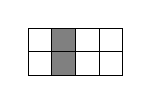
\begin{tikzpicture}
			\draw[] (0.6,-0.6) rectangle ++(0.3,0.3);
			\draw[fill=gray] (0.3,-0.6) rectangle ++(0.3,0.3);
			\draw[] (0.9,-0.6) rectangle ++(0.3,0.3);
			\draw[] (0,-0.6) rectangle ++(0.3,0.3);
			\draw[] (0,-0.3) rectangle ++(0.3,0.3);
			\draw[fill=gray] (0.3,-0.3) rectangle ++(0.3,0.3);
			\draw[] (0.6,-0.3) rectangle ++(0.3,0.3);
			\draw[] (0.9,-0.3) rectangle ++(0.3,0.3);
	\end{tikzpicture}}
	child[blue] {node[black] {\gam{1}{}}}
	child[blue] {node[black] {\gam{1}{{-}1}}}
	child[red, dashed] {node[black] {\gam{{-}1}{1}}}
}
child[blue] {node[black] {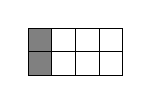
\begin{tikzpicture}
			\draw[] (0.6,-0.6) rectangle ++(0.3,0.3);
			\draw[] (0.3,-0.6) rectangle ++(0.3,0.3);
			\draw[] (0.9,-0.6) rectangle ++(0.3,0.3);
			\draw[fill=gray] (0,-0.6) rectangle ++(0.3,0.3);
			\draw[fill=gray] (0,-0.3) rectangle ++(0.3,0.3);
			\draw[] (0.3,-0.3) rectangle ++(0.3,0.3);
			\draw[] (0.6,-0.3) rectangle ++(0.3,0.3);
			\draw[] (0.9,-0.3) rectangle ++(0.3,0.3);
	\end{tikzpicture}}
	child[blue] {node[black] {\gam{1}{}}}
	child[blue] {node[black] {\gam{1}{{-}1}}}
	child[red, dashed] {node[black] {\gam{{-}1}{0,1}}}
}
child[red, dashed, level distance=80pt] {node[black, solid] { 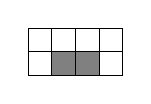
\begin{tikzpicture}
			\draw[fill=gray] (0.6,-0.6) rectangle ++(0.3,0.3);
			\draw[fill=gray] (0.3,-0.6) rectangle ++(0.3,0.3);
			\draw[] (0.9,-0.6) rectangle ++(0.3,0.3);
			\draw[] (0,-0.6) rectangle ++(0.3,0.3);
			\draw[] (0,-0.3) rectangle ++(0.3,0.3);
			\draw[] (0.3,-0.3) rectangle ++(0.3,0.3);
			\draw[] (0.6,-0.3) rectangle ++(0.3,0.3);
			\draw[] (0.9,-0.3) rectangle ++(0.3,0.3);
	\end{tikzpicture}}
	child[blue, solid] {node[black] {\gam{{-}1}{0, 1}}}
	child[red] {node[black] {\gam{1}{}}}
	child[red] {node[black] {\gam{0}{0}}}
}
child[red, dashed] {
	node[black, solid] { 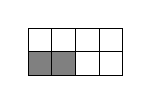
\begin{tikzpicture}
	\draw[] (0.6,-0.6) rectangle ++(0.3,0.3);
	\draw[fill=gray] (0.3,-0.6) rectangle ++(0.3,0.3);
	\draw[] (0.9,-0.6) rectangle ++(0.3,0.3);
	\draw[fill=gray] (0,-0.6) rectangle ++(0.3,0.3);
	\draw[] (0,-0.3) rectangle ++(0.3,0.3);
	\draw[] (0.3,-0.3) rectangle ++(0.3,0.3);
	\draw[] (0.6,-0.3) rectangle ++(0.3,0.3);
	\draw[] (0.9,-0.3) rectangle ++(0.3,0.3);
	\end{tikzpicture}}
		child[blue, solid] {node[black] {\gam{{-}1}{1}}}
		child[blue, solid] {node[black] {\gam{{-}1}{0,1}}}
		child[red] {node[black] {\gam{}{{-}1}}}
	}
;

\end{tikzpicture}
\end{center}
\end{figure}